
%%%
% Any line that begins with a percent symbol is a comment. To compile
% this document and view the output:
%
% Run Latex
% Run Bibtex
% Then run Latex twice.
%
% This should produce the output PDF file named main.pdf
%%%

% This defines the style to use for this document.
% Do not modify.
\documentclass[letterpaper]{article}

% The following are akin to "import" statements in Python or Java -
% these import useful commands into the document for you to use.  You
% don't have to modify any of these lines. The AAAI package formats
% this document in the style of submissions to the American
% Association for Artificial Intelligence conference, one of the top
% AI conferences in the world. You will find that many academic
% publications in AI use this format.
\usepackage{aaai} 
\usepackage{times} 
\usepackage{helvet} 
\usepackage{courier} 
\setlength{\pdfpagewidth}{8.5in} 
\setlength{\pdfpageheight}{11in} 
\usepackage{amsmath}
\usepackage{amsthm}
\usepackage{graphicx}
\usepackage{graphics}
\usepackage{moreverb}
\usepackage{subfigure}
\usepackage{epsfig}
\usepackage{txfonts}
\usepackage{algpseudocode}
\usepackage{multirow, multicol}
\usepackage{url}
\def\UrlBreaks{\do\/\do-}
\usepackage{tablefootnote}
\usepackage{color}

\setcounter{secnumdepth}{1}
\nocopyright

% Fill in your paper title, names and emails below
% The "\\" is used to break lines. The \url command
% is useful for typesetting URLs and email addresses (it uses the
% Courier font).
\title{Predicting Popularity of News Articles Using Machine Learning}
 \author{Huseyin Altinisik \and Chuxuan Yang\\
 \url{{hualtinisk, soyang}@davidson.edu}\\
 Davidson College\\
 Davidson, NC 28035\\
 U.S.A.}

% This is the "true" start of the document. All the text in your
% write-up should be placed within the \begin{document} and
% \end{document} decorators.
\begin{document}

\maketitle % formats the title nicely, do not modify

% While at this point you could just begin your write-up, often, it's
% useful to write each section of your write-up in a separate tex
% file (not unlike the modular decomposition you do for code you
% write). These \input commands insert the contents of the
% specified tex files in the order specified. Every write-up you
% submit must contain the following sections, in the shown order. Open
% each of the indicated tex files to understand what goes in each
% section, as well as for more TeX tips.

% Place the contents of your abstract between the
% \begin{abstract} and \end{abstract} decorators.

\begin{abstract}

This project focused on using machine learning to predict the popularity of a given piece of news article using existing datasets. In this project, we tested three regression models: \texttt{Linear Support Vector Regression}, \texttt{Random Forest Regressor} (RFR), and \texttt{Lasso Regression}. After conducting a series of experiments using these models, we ranked their performances based on the results of news article popularity prediction. We found that \texttt{LinearSVR} performed the best, with an r2 score of over $0.8$. This was true for both articles from ``Moreover" and ``Opoint", our two major data source. The best model used a combination of grid search with cross-validation. We think this project can be used to support the media and entertainment industry's efforts in producing contents that generate high volumes of readers, and can help many businesses better understand readers' interest.
\end{abstract}



% The \section{} command formats and sets the title of this
% section. We'll deal with labels later.
\section{Introduction}
\label{sec:intro}

About fifty years ago, reading in paper copies through subscriptions was the only choice for many families. However, as technology advances, digital reading has gained tremendous popularity among the younger generations. According to the Fortune Magazine, today $85\%$ adults in the US read news on their mobile devices. Therefore, it is in news medias' commercial interests to know which of their articles generate the most attention from the readers.\\ 

For this project, we set out to use machine learning techniques to predict popularity of a news article based on its text content. Our dataset contains over $12000$ articles from different websites, covering a wide range of topics. Some articles have a ``momentum" score, which signals its popularity among readers. The momentum scores range from $0$ to $6448.06$; for this project, we assumed that the higher the momentum score, the more popular the article. To turn our source data into usable feature data for this project, we performed text data pre-processing using \texttt{pandas}, as well as feature extraction using \texttt{TfidfVectorizer} from the \texttt{scikit-learn} library\cite{scikit-learn}. We then trained our models using \texttt{scikit-learn}'s built-in \texttt{LinearSVR}, \texttt{RandomForestRegressor}, and \texttt{Lasso Regression} models on articles that carry momentum scores. We will explain in greater details for each step in later sections, including our results in model performances.\\

In the next section, we will talk about preparing our data prior to training them on any models. 

% Citations: As you can see above, you create a citation by using the
% \cite{} command. Inside the braces, you provide a "key" that is
% uniue to the paper/book/resource you are citing. How do you
% associate a key with a specific paper? You do so in a separate bib
% file --- for this document, the bib file is called
% project1.bib. Open that file to continue reading...

% Note that merely hitting the "return" key will not start a new line
% in LaTeX. To break a line, you need to end it with \\. To begin a 
% new paragraph, end a line with \\, leave a blank
% line, and then start the next line (like in this example).




\section{Background}
\label{sec:background}

\subsection{Data Pre-Processing \& Feature Extraction}
The raw data for this project are stored in two large parent gzip files, ``Moreover" and ``Opoint". The Opoint parent  gzip file originally contained 2679 child gzip files, whereas the Moreover parent file contained 12420 child gzip files. Each child gzip file stores an ``.xml" file. Inside each ``.xml" file we found a  different number of articles, including meta data such as its unique article ID, the author, the source of the article, as well as the article content, which we considered to be our feature for this project. We also had a csv file called ``Momentum" that stores the article IDs as well as its matching momentum scores for some of the articles from our file source. \\

Our first task was to iterate over each article inside the folders and the ``.xml" files ,and consolidate all articles with a momentum score into a new CSV file for model training purposes. To do so, we iterated over all articles inside the Moreover files and extracted the contents for articles with an ``id\_article" that can be found in ``Momentum.csv". For the Opoint files, we iterated over the files and saved contents for articles with a matching ``feed\_article\_id" that exists in the Momentum csv file. We realized after finishing this step that our output csv file had a few empty or unusually structured rows; and since our data size is large enough, we decided to discard those rows. \\
Because text data cannot be fed directly to the algorithms themselves as most of them expect numerical feature vectors with a fixed size rather than the raw text documents with variable length, we decided to perform feature extraction using the \texttt{TfidfVectorizer}. The \texttt{TfidfVectorizer} takes in individual articles in string formats, tokenizes the article strings into words and gives an integer id for each possible token or word by using white-spaces and punctuation as token separators. The vectorizer then counts the occurrences of tokens in each article and essentially normalizes the dataset.\\
Through this process, each individual token occurrence frequency (normalized or not) is treated as a feature, and the vector of all the token frequencies for a given document is considered a multivariate sample.

\subsection{Feature Modification}
We realized at the early stages of our project that for large article texts, some words will be very present (e.g. “the”, “it”, “a” in English) hence carrying very little meaningful information about the actual contents of the article. If we were to feed the data on frequency directly to a model, those very frequent terms would potentially shadow the frequencies of rarer yet more interesting terms. Hence, we defined a list of stop words prior to running any models. Our list of words looks like this: ['the', 'a', 'is','are','for','that','as','it','to','be'].\\
Later in our experiments, it occurred to us that our CSV files had many duplicated articles with the exact same contents. For example, our sample size before we deleted any duplicates for articles from Moreover was $2354$, and after we dropped all samples that have the same titles, we had only $1164$ samples left. We will discuss our results later in this paper.  












\section{Models \& Experiments}
\label{sec:expts}
For this project, we decided to use the following three models:
\subsection{Linear SVR}
  Short for Linear Support Vector Regression, this model is similar to the Support Vector Regression model, with the parameter kernel = `linear'. According to \texttt{scikit-learn}, \texttt{LinearSVR} is implemented in terms of liblinear rather than libsvm, hence it has more flexibility for the choice of penalties and loss functions, and can scale better to large numbers of samples. 
  \begin{itemize}
      \item Hyperparameters
  \begin{enumerate}
    \item C parameter (default = $1.0$)\\
    For this model, we first ran 10-folds cross validation on the C parameter, which stands for penalty for the error term. We implemented the model with L2 penalty. Since the bigger the C value, the less regularization is used, we expected to see an improvement in model performance as C increased.
    \item loss (default = L1)\\
    The default setting for the loss function is L1, the ``epsilon-insensitive" loss. After getting poor cross validation performance from this setting, we changed the loss setting to be L2, the ``squared epsilon-insensitive". Following this tuning, we immediately saw a significant increase in our model results.
    \end{enumerate}
    \item Result Metric\\
    For LinearSVR, we looked at the r2 score as an indication of model performance. The r2 score is a statistic measure that tells the fitness of a model. A score of $1$ indicates that the regression line perfectly fits the data. \\
 \end{itemize}
\subsection{Random Forest Regressor}
This model creates a diverse set of classifiers by introducing randomness in the tree construction process. Because of such randomness, we expected the bias and variance of this model to be slightly higher. The model fits a number of decision trees on the sub-samples of the data set, and uses averaging to improve accuracy scores and to prevent over-fitting. Therefore, we expected it to yield an overall well-performed model. 
\begin{itemize}
      \item Hyperparameters
  \begin{enumerate}
    \item n\_estimators (default = $10$)\\
    This represents the number of trees in a forest. We ran CV on this parameter first with values $[5,10,15,20,25]$, then with $[50,100,150,200,250]$, on top of the 10-folds cross validation we also performed on the model.
    \item max\_features (default = n\_features)\\
    This indicates the number of features to consider when looking for the best split. For our project, we first set max\_feature to be the number of features we have for each article: the number of columns in our data frame. We also tried setting it to be 'sqrt' and 'log2', in which case max\_features=sqrt(n\_features) and max\_features=log2(n\_features).
    \item max\_depth (default = None)\\
    This parameter represents the maximum depth of the tree. We left this setting as it was, because we wanted for all the nodes to expand till all leaves are pure. 
     \item min\_samples\_split (default = 2)\\
    This stands for the minimum number of samples required to split an internal node. We also used the default setting of $2$.
    \end{enumerate}
    \item Result Metric\\
    The performance of the Random Forest Regression was also measured using r2 scores.\\
 \end{itemize}
\subsection{Lasso Regression}
 Lasso is a regularization technique that works by penalizing the magnitude of feature coefficients to minimize the amount of error between the predictions and actual observations. Lasso performs L1 regularization, which is the sum of the weights in the loss function. Lasso shrinks the less important feature’s coefficient to zero, which works well for feature selection when we have a huge number of features as in our case. 
\begin{itemize}
    \item Hyper-parameters
\begin{enumerate}
    \item alpha \\
    The alpha parameter is a constant value that is multiplied by the L1 term. The higher the alpha value, the stronger the penalization. If the alpha value is $0$, the Lasso regression will result in the same coefficients as a linear regression \cite{ChrisAlbon}. The alpha values we tuned for this projects were $[0.001,0.002,0.005,0.01,0.02,0.05,0.1,0.2,0.5,1,2,5]$.
  \end{enumerate}
  \item Result Metric\\
     The Lasso Regression performance was calculated using the r2 scores. 

 \end{itemize}
 In the next section, we will discuss our results for the models. 
  
  


\section{Results}
\label{sec:results}
Our results are displayed in Figure $1$.
\begin{figure}[htb]
  \centering % centers the entire table

  % The following line sets the parameters of the table: we'll have
  % three columns (one per 'c'), each
  % column will be centered (hence the 'c'; 'l' or 'r' will left or
  % right justify the column) and the columns
  % will have lines between them (that's the purpose of the |s between
  % the 'c's).
  \begin{tabular}{|c|c|c|} 
    \hline \hline % draws two horizontal lines at the top of the table
    \textbf{Model Settings} & \textbf{Moreover} & \textbf{OPoint} \\ % separate column contents using the &
    \hline % line after the column headers
    LinearSVR, L1 & $-0.059$ & $-0.034$ \\
    Linear SVR, L2 & $0.826$ & $0.860$\\
    RFR, max\_feature = 'None' & $0.125$ & $0.373$ \\
    RFR, max\_feature = 'sqrt' & $0.263$ & $0.350$ \\
    RFR, max\_feature = 'log2' & $0.096$ & $0.337$ \\
    Lasso regression & $0.554$ & $-0.435$ \\
    \hline \hline
  \end{tabular}

  % As with figures, *every* table should have a descriptive caption
  % and a label for ease of reference.
  \caption{Results under 10-folds Cross Validation}
  \label{tab:example}

\end{figure}
For \texttt{LinearSVR}, the r2 score improved substantially after we switched from L1 to L2 penalty. We think this is because the L2 penalty led to lower regularization strength. For the different C values we tested, $1.5$ turned out to be the one that gave us the best result among all. \\
For \texttt{RandomForestRegressor}, we started out using a smaller number of trees, ranging from $5$ to $25$ trees. However, our initial r2 scores from \texttt{RFR} yielded extremely high variance, ranging from $0.249$ to $-4.88$. We realized that this was correlated to the smaller number of trees we had, so we increased our tree size substantially. Our results can be seen from the figure above, and a number of $150$ and $200$ trees seemed to consistently generated the best results.\\
Overall, our models still had relatively high variance in results. Under the $10$-folds cross validation we performed for \texttt{RFR} and \texttt{LinearSVR} for example, we saw that the r2 scores could still range from as low as $-0.257$ to as high as $0.989$. Figure $2$ below visualizes one example of such variance. We thought this was because we had way too many features to deal with in this project, and this substantially increased the randomness of the results. For both \texttt{RandomForestRegressor} and \texttt{LinearSVR}, the results are also low-biased. We assumed the high variance, low bias combination happened because there were too many decision nodes to go through before each model could arrive at a result. Because of this, even a small change in input variable could result in completely different regression models, hence leading to the phenomenon that we observed.\\
\begin{figure}[htb]

  \centering  % centers the image in the column

  % replace the second argument below with your filename. I like to
  % place all my figures in a sub-directory to keep things organized
  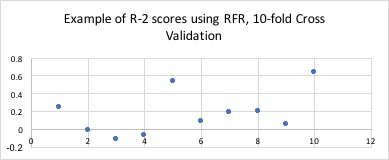
\includegraphics[width=0.47\textwidth]{1.jpg}

  % *Every* figure should have a descriptive caption.
  \caption{Results of R-2 scores derived from the RFR model, using n\_estimator = $100$, max\_feature = 'sqrt' and max\_depth = $20$. }

  % The label is a handle you create so that you can refer to this
  % figure (using the \ref{} command) from other parts of your
  % document. LaTeX automatically renumbers figures and updates
  % references when you recompile, so you should do it this way rather
  % than hard-coding in references. Notice that I've also been
  % creating labels for the various sections in the document; I could
  % use \ref{} command to refer to those sections using their labels
  % too.
  \label{fig:tex}
\end{figure}

The overall performance of the Lasso regression on our dataset was fairly good for articles from Moreover, but not as satisfactory for articles from Opoint. The scores obtained after a 10-fold cross validation and hyper-parameter tuning on alpha did not lead to remarkable improvement. In general, we expected that hyper-parameter tuning on alpha would enhance the performance of the model, since using smaller alpha values reduces the amount of penalization \cite{AnalyticsVidhya}; however, the results obtained after cross validation proved that \textttt{Lasso} performed better than \texttt{RFR} on the Moreover articles, and it performed significantly worse on the articles from Opoint. 

As mentioned in the previous sections, later on in our project we realized that without deleting duplicates in our data frame, we were essentially overestimating our model performance, since we were testing the model on what it was trained on. The results we delivered in Figure $1$ were recorded after we had deleted the duplicates. We compared the two sets of results before and after we discarded duplicates, and the results are shown in Figure $3$. Interestingly, \texttt{RFR} was affected a lot more than \texttt{LinearSVR} was, perhaps due to the fact that \texttt{LinearSVR} is well-performed for text analytics problem to begin with. However, keeping duplicates simply would create excessive optimism for \texttt{RFR}'s model performances. 
\begin{figure}[htb]

  \centering  % centers the image in the column

  % replace the second argument below with your filename. I like to
  % place all my figures in a sub-directory to keep things organized
  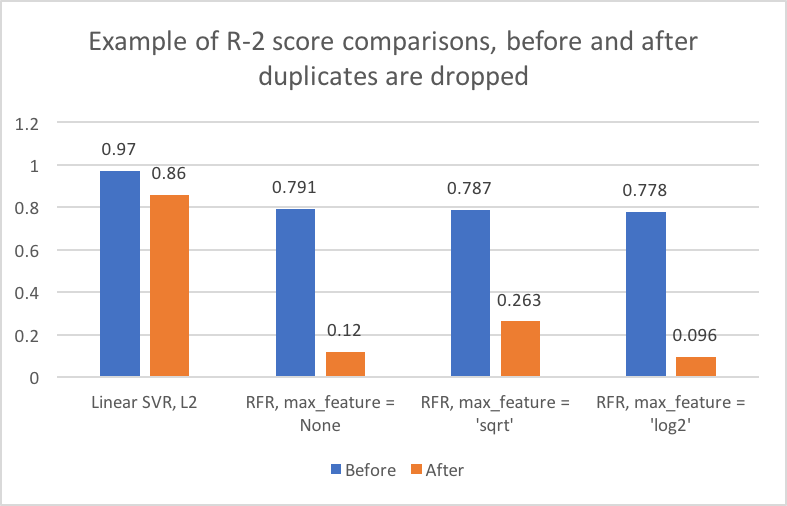
\includegraphics[width=0.47\textwidth]{2.png}
 \caption{Visualization of the effects after duplicates were dropped}
  % *Every* figure should have a descriptive caption.
  % The label is a handle you create so that you can refer to this
  % figure (using the \ref{} command) from other parts of your
  % document. LaTeX automatically renumbers figures and updates
  % references when you recompile, so you should do it this way rather
  % than hard-coding in references. Notice that I've also been
  % creating labels for the various sections in the document; I could
  % use \ref{} command to refer to those sections using their labels
  % too.
  \label{fig:tex}

\end{figure}






\section{Conclusions}
\label{sec:concl}

In this paper, we set out to build a model that could accurately predict the popularity of news articles in terms of momentum scores. After converting text data in to trainable,numerical values, we built and trained our models, and  discovered that \texttt{LinearSVR} came away with the best results.Our most important discovery is that increasing the number of trees in the \texttt{RandomForestRegressor} model mitigated the high variance problem we saw in our previous results by a fair amount. Perhaps using a large number of trees is required for this problem, given the immense feature size we had.\\


Should we have more time in the future, we would like to go a few steps further with pre-processing our data. First of all, we would like to add a few meta data properties to be the feature data. Recall that for this project, we only considered the text content of individual articles as our feature. However, meta data such as the specific website where an article is published, its author, or even the time it was published can potentially affect its popularity too. Secondly, we would like to make sure all duplicates are deleted for a less biased result. The \texttt{panda}'s drop\_duplicates function allowed us to throw away articles that have the same titles. However, we found out later in our project that this approach didn't do the entire job as some articles had the exact same contents and momentum scores, but had different titles. Lastly, we would trim down our data set even more and take away more words that do not contribute to the popularity measure. For this project, we only took out common English words like ``a, the, it", etc. However, we believe that only a small number of words should matter for the popularity measure, and sometimes only one keyword such as \textit{Donald} could be responsible for a high score. \\


\section{Contributions}
\label{sec:contrib}

Huseyin and Sophie worked on the pre-processing of the data and wrote the code for \texttt{LinearSVR} and \texttt{RandomForestRegressor}, and \texttt{Lasso Regressor}. For the paper, Sophie wrote the Abstract, Introduction, and Background. Both partners wrote the Experiment, Results, and the Conclusion sections together. Both partners proof-read before submitting the paper. 



\section{Acknowledgements} 
\label{sec:ack} 

We would like to thank Quoin, the Charlotte based data science company for providing the dataset for our project, as well as Dr.  Ramanujan for helping us interpret the datasets. We would also like to thank our friends and classmates for their generous encouragement and support throughout the project.


% This creates the references section. Open the project1.bib file to
% see how to organize your references.
\bibliography{project1}
\bibliographystyle{aaai} % sets citation and bib style, do not modify

\end{document}
